\documentclass{beamer}

%\beamertemplatenavigationsymbolsempty
%\setbeamerfont{page number in head/foot}{size=\small}
%\setbeamertemplate{footline}[frame number]
%\usefonttheme[onlymath]{serif}

\usepackage[utf8]{inputenc}

\usepackage[T1]{fontenc}
\usepackage[english]{babel}
%\usepackage[utf8]{inputenc}

\usepackage{tikz}
\usetikzlibrary{calc}
\usetikzlibrary{arrows, backgrounds}
\usetikzlibrary{matrix, arrows.meta}
\usetikzlibrary{decorations.pathreplacing}
\usetikzlibrary{positioning, fit, shapes}

%\usetikzlibrary{external}
%\tikzexternalize[prefix=tikz/]

\newcommand{\backupbegin}{
   \newcounter{finalframe}
   \setcounter{finalframe}{\value{framenumber}}
}
\newcommand{\backupend}{
   \setcounter{framenumber}{\value{finalframe}}
}

% Scale all pgf plots, not only coordinates
\usepackage{adjustbox}

%\usepackage{amsfonts}
%\usepackage{amsmath}
%\usepackage{amsthm}
\usepackage{bm}

\usepackage{pgfplots}
\pgfplotsset{compat=1.16}
\usepgfplotslibrary{groupplots}

% Used for split environment
\usepackage{amsmath}
% Separate rows in align environment by this amount
\addtolength{\jot}{1em}

\usepackage{graphicx}
\graphicspath{{../fig/} {fig/}}
\usepackage{subfig}
\usepackage{wrapfig}

% Clickable links
\usepackage{hyperref}
\hypersetup{
	colorlinks,
	citecolor=black,
	filecolor=black,
	linkcolor=black,
	urlcolor=black
}

\usepackage[pdf]{graphviz}

%\usepackage[dvipsnames]{xcolor}
\usepackage{listings}

\lstset{
	language=c,
  basicstyle=\small\ttfamily,  % the size of the fonts that are used for the code
	numbers=none,                   % where to put the line-numbers
  inputencoding=latin1,
  numberstyle=\tiny,  % the style that is used for the line-numbers
  stepnumber=1,                   % the step between two line-numbers. If it's
				    %1, each line 
                                  % will be numbered
  %numbersep=5pt,                  % how far the line-numbers are from the code
  backgroundcolor=\color{white},      % choose the background color.
  showspaces=false,               % show spaces adding particular underscores
  showstringspaces=false,         % underline spaces within strings
  showtabs=false,      % show tabs within strings adding particular underscores
	frame=none,                   % adds a frame around the code
  rulecolor=\color{black},        % if not set, the frame-color may be changed
				   % on line-breaks within not-black text (e.g.
				   % comments (green here))
	tabsize=6,                      % sets default tabsize to 2 spaces
  columns=fullflexible,
  extendedchars=true,
  captionpos=b,                   % sets the caption-position to bottom
  breaklines=true,                % sets automatic line breaking
  breakatwhitespace=false,        % sets if automatic breaks should only happen
				    %at whitespace
  title=\lstname,                   % show the filename of files included with
				    %\lstinputlisting;
                                  % also try caption instead of title
  keywordstyle=\color{blue},          % keyword style
	commentstyle=\color{gray},       % comment style
	stringstyle=\color{brown},         % string literal style
	escapeinside={|*}{*|},            % if you want to add LaTeX within your code
	morecomment=[l][\color{purple}]{\#},
	moredelim=[il][\color{purple}]{@},
	abovecaptionskip=-15pt
%	belowcaptionskip=-15pt
}


\usepackage{csquotes}

\usepackage{siunitx}

\usepackage{multicol}

\usepackage{epigraph}
\setlength{\epigraphwidth}{0.7\textwidth}

\usepackage{caption}
\captionsetup{font=footnotesize}

% Macros para ayudar a la redacción
% Vector
\newcommand*\mat[1]{ \begin{pmatrix} #1 \end{pmatrix}}
\newcommand*\arr[1]{ \begin{bmatrix} #1 \end{bmatrix}}
\newcommand*\V[1]{\bm{#1}}
\newcommand{\E}{\V{E}}
\newcommand{\rhog}{\rho_\text{ghost}}
\newcommand{\F}{\V{F}}
\newcommand{\B}{\V{B}}
\renewcommand*{\v}{\V{v}}
\newcommand{\x}{\V{x}}
\newcommand{\dt}{\Delta t}
\newcommand{\dx}{\Delta x}
\newcommand*\neigh[1]{\mathcal{N}(#1)}

% Norm
\newcommand\norm[1]{\left\lVert#1\right\rVert}

%\title{Particle-in-cell plasma simulation\\with OmpSs-2}
%\author{Rodrigo Arias Mallo\\
%\vspace{1em}
%{\footnotesize Director: Vicenç Beltran Querol \\
%Tutor: Jordi Torres Viñals}}
%\institute{Universitat Politècnica de Catalunya (UPC)}
%\date{\today}









% Running style for the nodes
\tikzset{
	running/.style={fill=green!30}
}

\tikzset{
	stopped/.style={fill=red!30}
}

\tikzset{
%	master/.pic = {
	pics/master/.style args={#1}{
		code={
			\matrix[
				ampersand replacement=\&,
				nodes={#1,draw,circle,inner sep=0mm,minimum size=8mm},
				column sep=5mm,
	%				left=1cm of O,
			] (t)
			{
				\node (t0) {$t_0$}; \&
				\node (t1) {$t_1$}; \&
				\node (t2) {$t_2$}; \&
				\node (t3) {$t_3$}; \\
			};

			\node[draw,fit=(t0) (t3),inner sep=1mm,rounded corners=4mm] (master) {};
			%\node[draw,fit=(t0) (t3),inner sep=0.5mm,ellipse] (master) {};

			\node[left=1mm of master] {Master process};
		}
	}
}
\tikzset{
%	master/.pic = {
	pics/master/.style args={#1}{
		code={
			\matrix[
				ampersand replacement=\&,
				nodes={#1,draw,circle,inner sep=0mm,minimum size=8mm},
				column sep=5mm,
	%				left=1cm of O,
			] (t)
			{
				\node (t0) {$t_0$}; \&
				\node (t1) {$t_1$}; \&
				\node (t2) {$t_2$}; \&
				\node (t3) {$t_3$}; \\
			};

			\node[draw,fit=(t0) (t3),inner sep=1mm,rounded corners=4mm] (master) {};
			%\node[draw,fit=(t0) (t3),inner sep=0.5mm,ellipse] (master) {};

			\node[left=1mm of master] {Master process};
		}
	}
}

\tikzset{
%	workers/.pic = {
	pics/workers/.style args={#1}{
		code={
			\matrix[
				ampersand replacement=\&,
				nodes={
					#1,
					double,
					double distance=1mm,
					draw,
					circle,
					inner sep=0mm,
					minimum size=8mm
				},
				column sep=5mm] (w) {
				\node (w0) {$w_0$}; \&
				\node (w1) {$w_1$}; \&
				\node (w2) {$w_2$}; \&
				\node (w3) {$w_3$}; \\
			};

			\node[right=1mm of w] {Workers};
		}
	}
}

\tikzset{
	cpus/.pic = {
		\matrix[
			ampersand replacement=\&,
			matrix of nodes,
			nodes={
				draw,
				rectangle,
				inner sep=0mm,
				minimum size=6mm
			},
			column sep=5mm
		] (c)
		{
			\node (c0) {$c_0$}; \&
			\node (c1) {$c_1$}; \&
			\node (c2) {$c_2$}; \&
			\node (c3) {$c_3$}; \\
		};

		\node[above=1mm of c] {CPUs};
	}
}


\tikzset{
	mem/.pic = {
		\matrix[
			nodes={
				anchor=center,
				draw,
				rectangle,
				minimum width=4cm,
				minimum height=1cm,
			},
			row sep =-\pgflinewidth,
			column sep = -\pgflinewidth,
			column sep=0mm
		] (m)
		{
			\node (m0) {$m_0$}; \\
			\node (m1) {$m_1$}; \\
			\node (m2) {$m_2$}; \\
			\node (m3) {$m_3$}; \\
		};

		\node[below=1mm of m] {Shared memory};
	}
}






\begin{document}

\begin{frame}[fragile]
\begin{figure}[h]
\begin{adjustbox}{max totalsize={\textwidth}{\textheight},center}
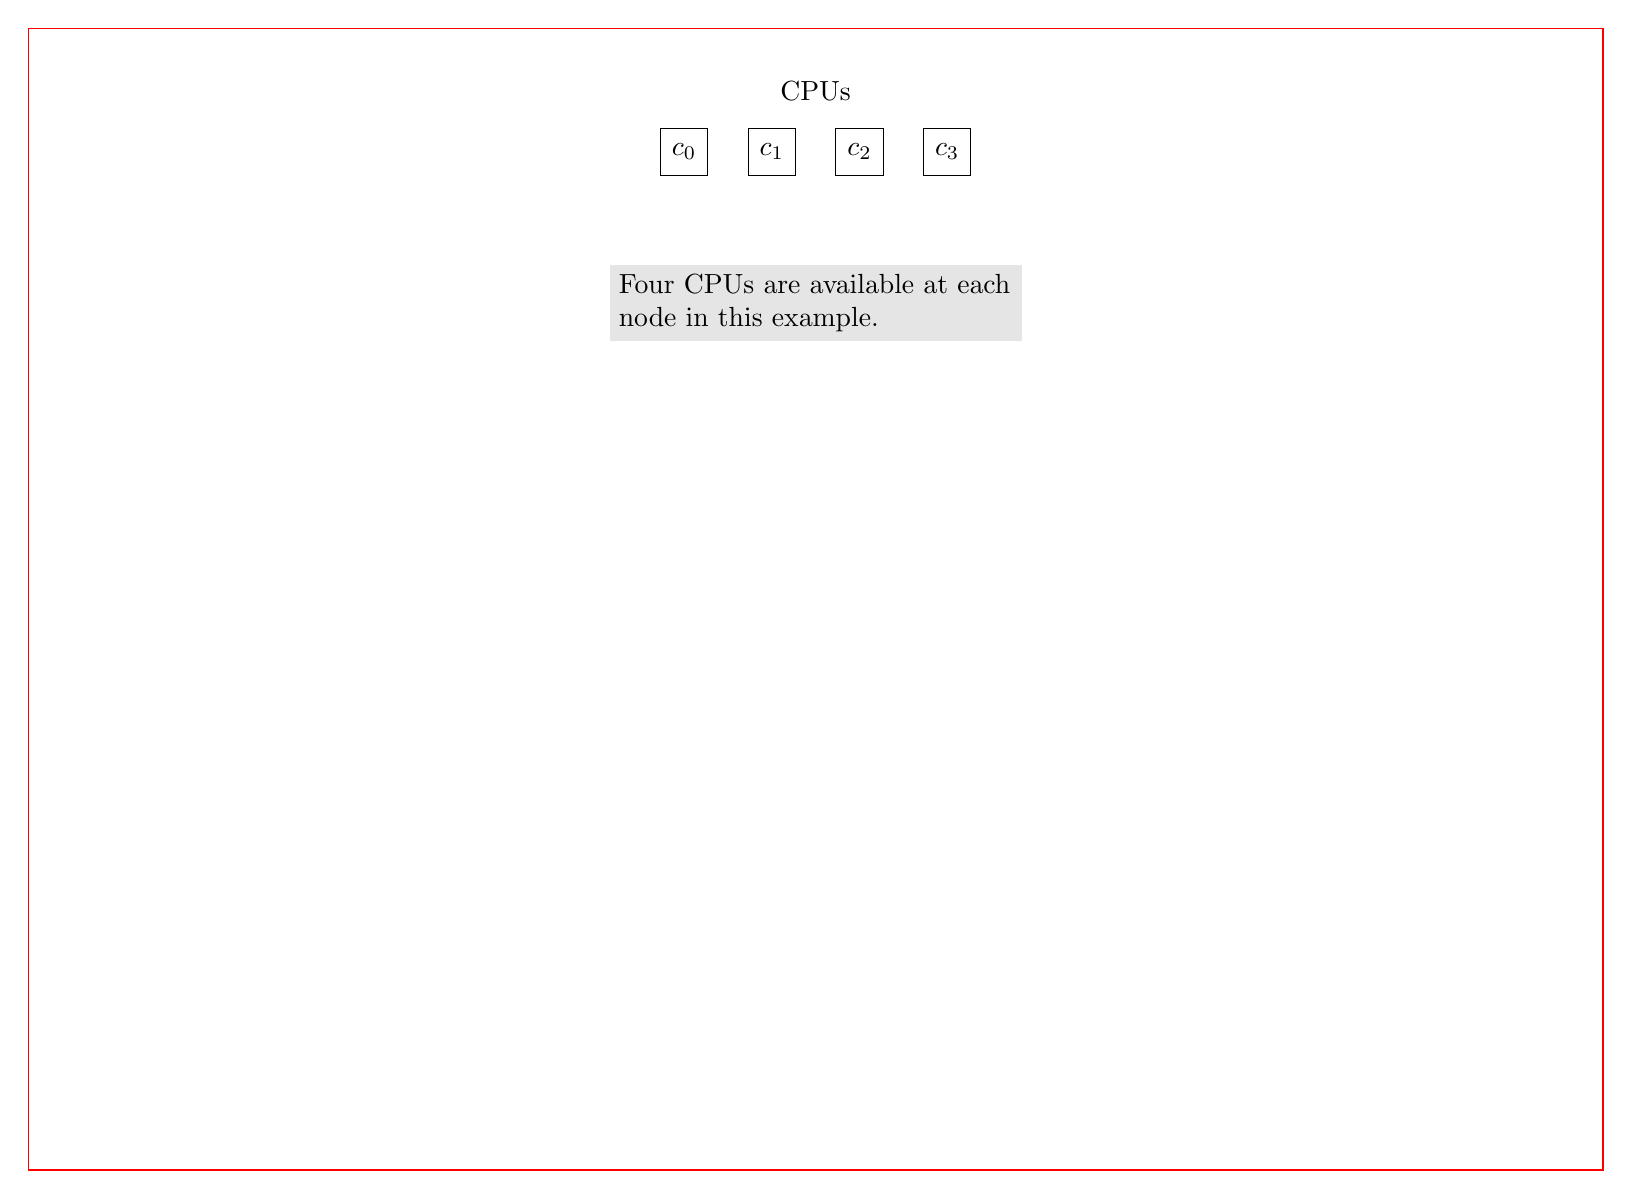
\begin{tikzpicture}[
		>=latex,
	]

	% The center will be the origin
	\coordinate (O) at (0,0);

	% Draw the canvas
	\draw[red] (-10,-8.5) rectangle (10,6);

	% Draw the CPUs
	\pic[above=4cm of O] {cpus};

	\node (text) [fill=gray!20,below=1cm of c,text width=5cm]
		{Four CPUs are available at each node in this example.};

%	\draw[->] (text) -- (c);
%	\draw[->] (text) -- (c0);
%	\draw[->] (text) -- (c1);
%	\draw[->] (text) -- (c2);
%	\draw[->] (text) -- (c3);

\end{tikzpicture}
\end{adjustbox}
\end{figure}
\end{frame}

\begin{frame}[fragile]
\begin{figure}[h]
\begin{adjustbox}{max totalsize={\textwidth}{\textheight},center}
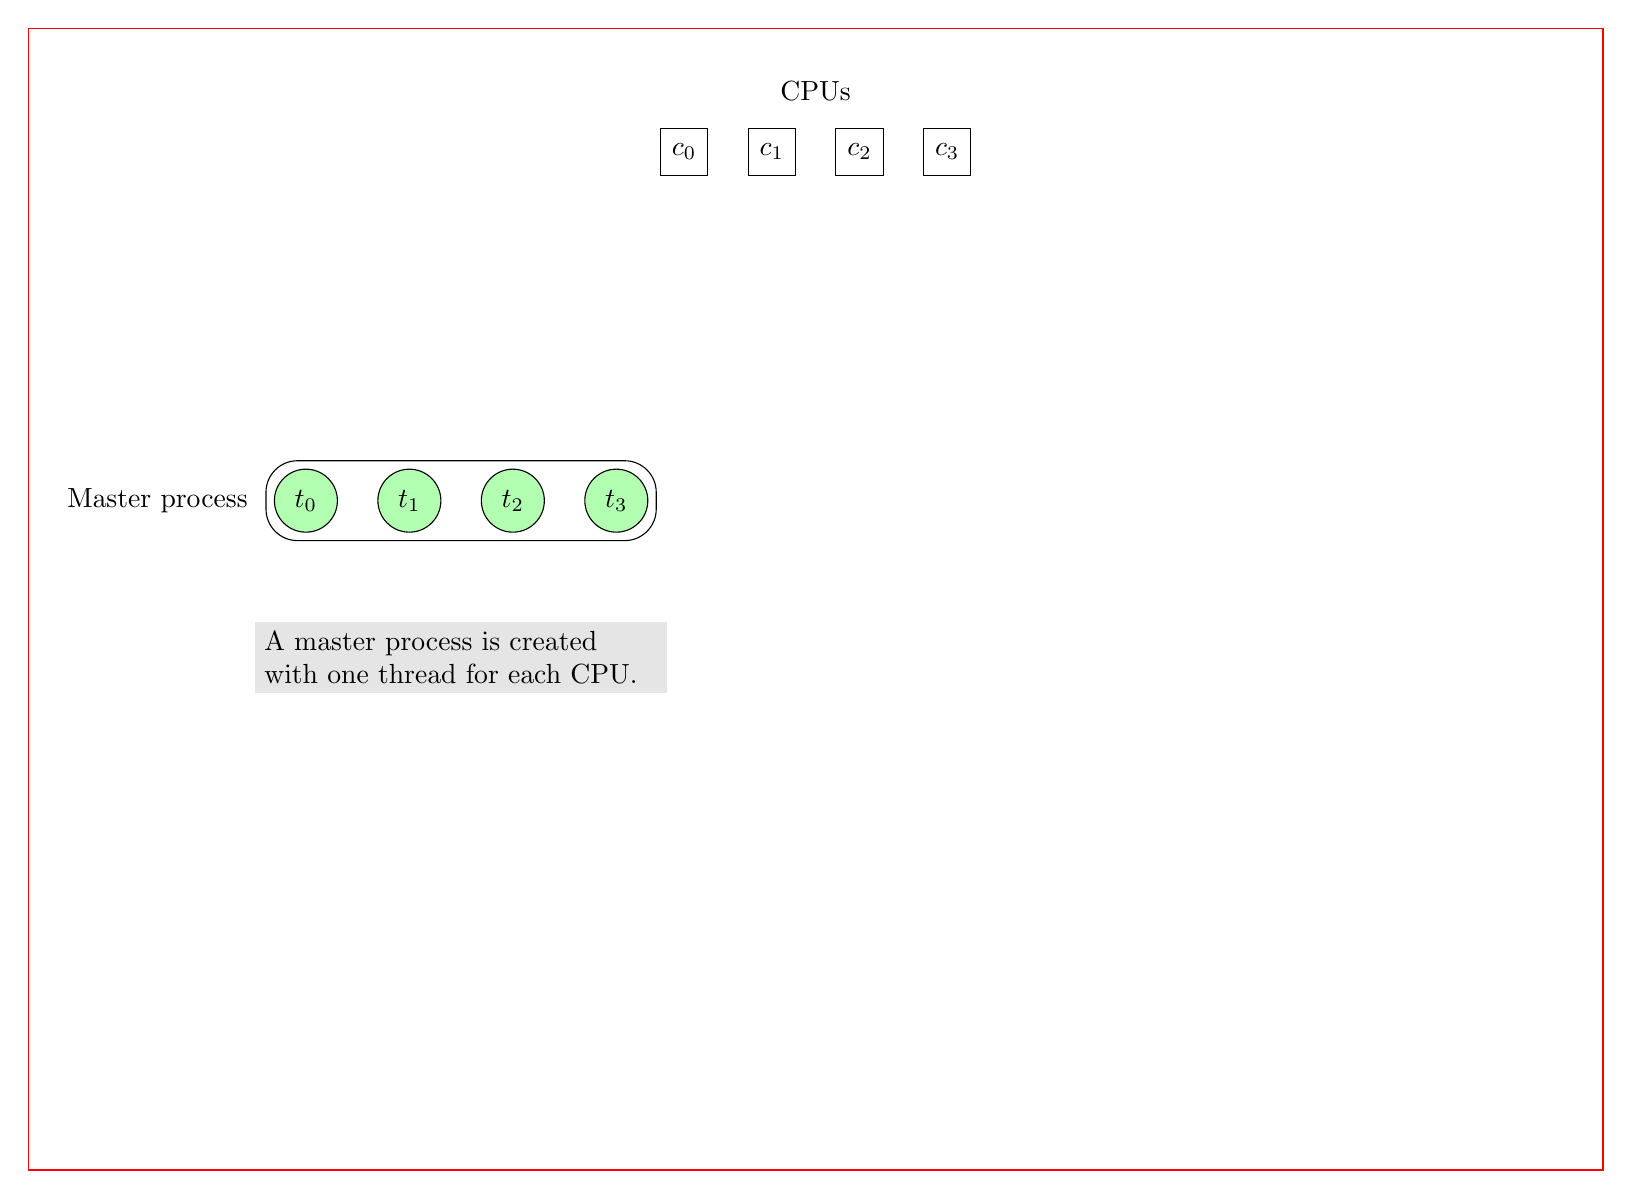
\begin{tikzpicture}[
		>=latex,
	]

	% The center will be the origin
	\coordinate (O) at (0,0);

	% Draw the canvas
	\draw[red] (-10,-8.5) rectangle (10,6);

	% Master process with 4 threads
	\pic[left=2cm of O] {master={running}};

	% Draw the CPUs
	\pic[above=4cm of O] {cpus};

	\node (text) [fill=gray!20,below=1cm of t,text width=5cm]
		{A master process is created with one thread for each CPU.};

\end{tikzpicture}
\end{adjustbox}
\end{figure}
\end{frame}

\begin{frame}[fragile]
\begin{figure}[h]
\begin{adjustbox}{max totalsize={\textwidth}{\textheight},center}
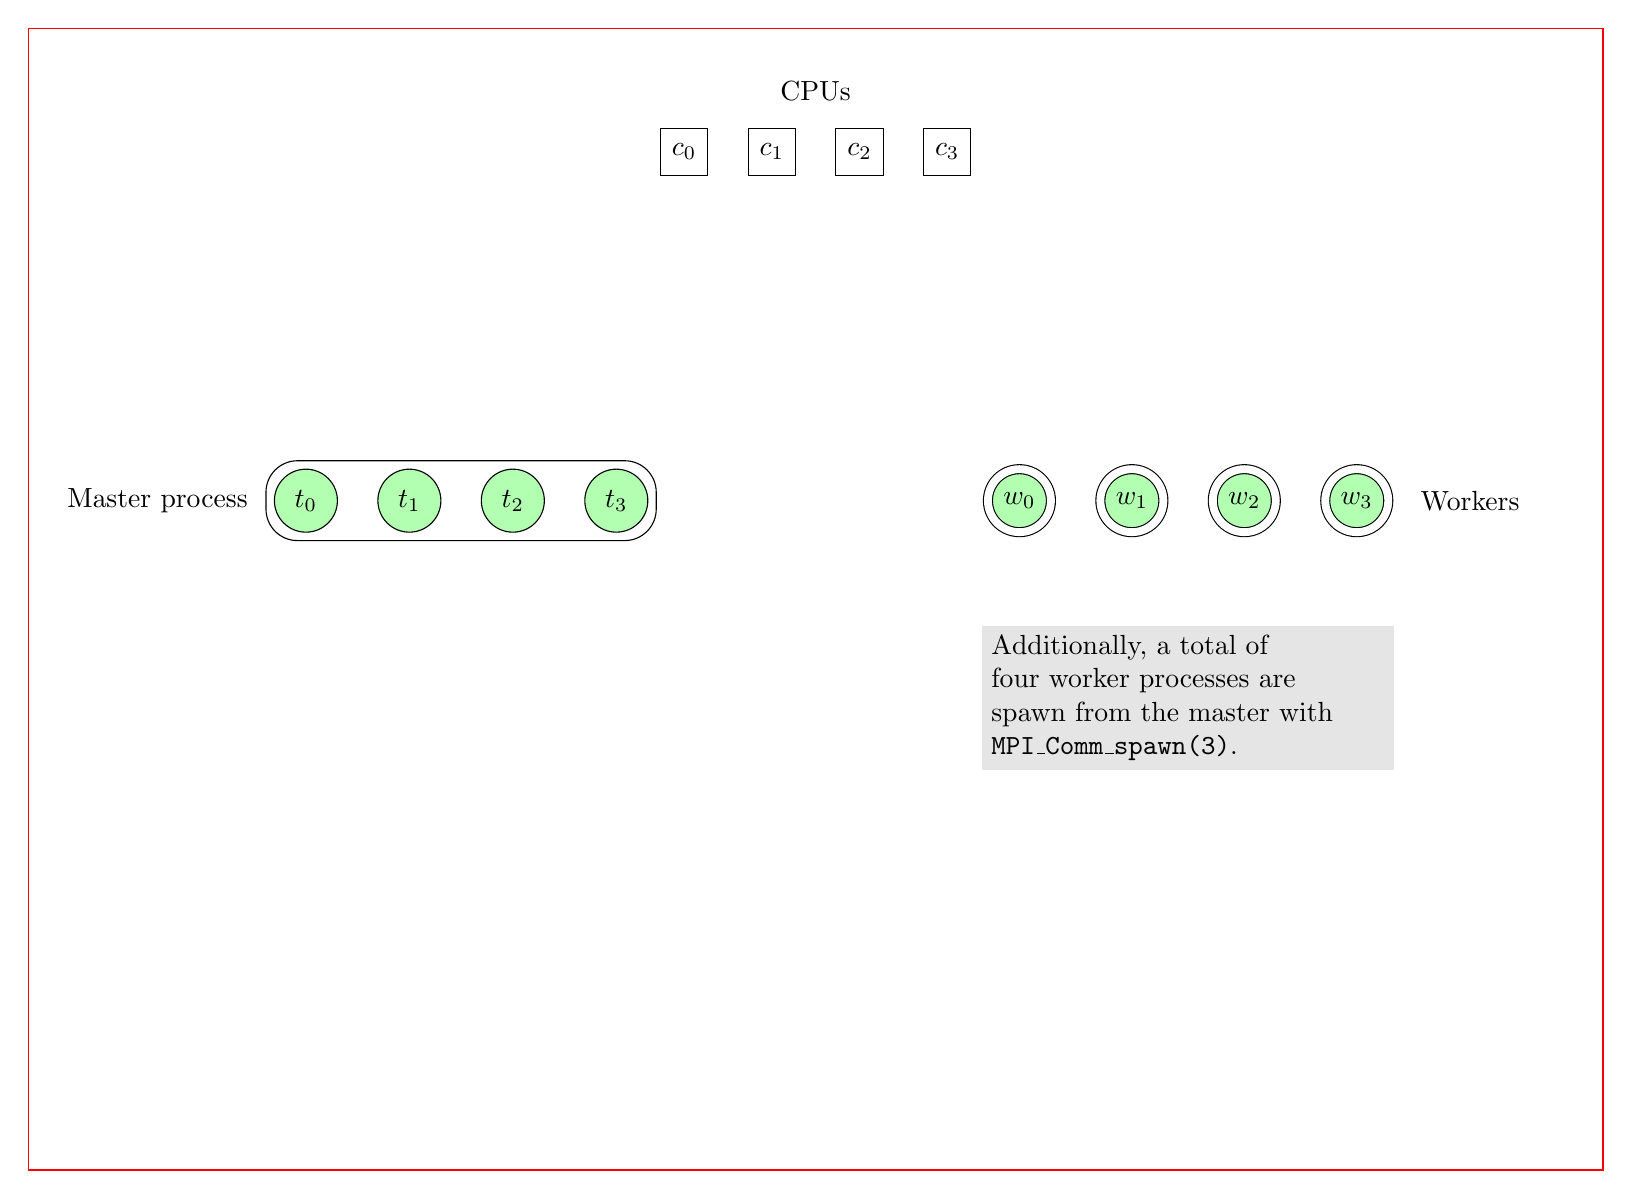
\begin{tikzpicture}[
		>=latex,
	]

	% The center will be the origin
	\coordinate (O) at (0,0);

	% Draw the canvas
	\draw[red] (-10,-8.5) rectangle (10,6);

	% Master process with 4 threads
	\pic[left=2cm of O] {master={running}};

	% Draw the CPUs
	\pic[above=4cm of O] {cpus};

	% Draw the workers
	\pic[right=2cm of O] {workers={running}};

	\node (text) [fill=gray!20,below=1cm of w,text width=5cm]
		{Additionally, a total of four worker processes are spawn from the master 
		with \texttt{MPI\_Comm\_spawn(3)}.};


\end{tikzpicture}
\end{adjustbox}
\end{figure}
\end{frame}

\begin{frame}[fragile]
\begin{figure}[h]
\begin{adjustbox}{max totalsize={\textwidth}{\textheight},center}
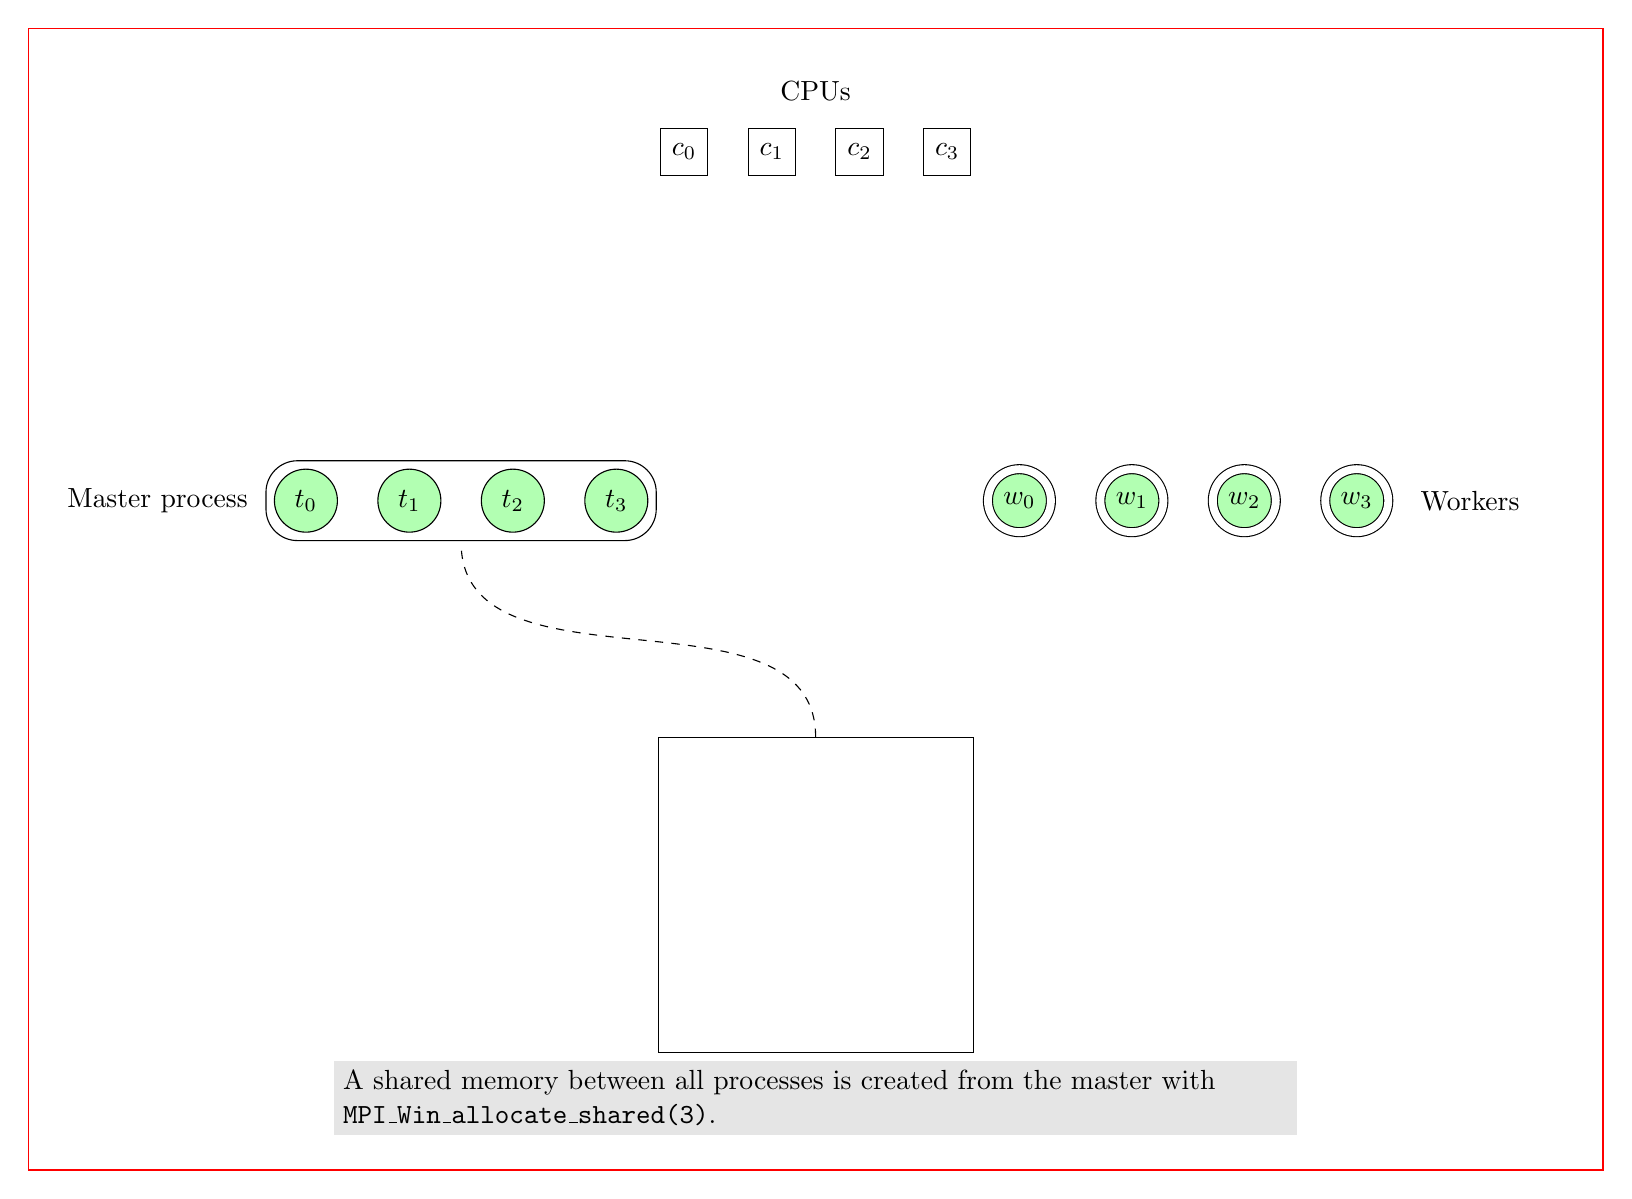
\begin{tikzpicture}[
		>=latex,
	]

	% The center will be the origin
	\coordinate (O) at (0,0);

	% Draw the canvas
	\draw[red] (-10,-8.5) rectangle (10,6);

	% Master process with 4 threads
	\pic[left=2cm of O] {master={running}};

	% Draw the CPUs
	\pic[above=4cm of O] {cpus};

	% Draw the workers
	\pic[right=2cm of O] {workers={running}};

	% Draw shared memory
	%\pic[below=3cm of O] {mem};

	\node[draw,
				minimum width=4cm,
				minimum height=4cm,
				below=3cm of O,
				] (m)	{};

	\node (text) [fill=gray!20,below=1mm of m,text width=12cm]
		{A shared memory between all processes is created from the master with 
		\texttt{MPI\_Win\_allocate\_shared(3)}.};

	% Draw lines from master to mem
	\draw[dashed] (m.north) to[out=90,in=-90] (t.south);


\end{tikzpicture}
\end{adjustbox}
\end{figure}
\end{frame}

\begin{frame}[fragile]
\begin{figure}[h]
\begin{adjustbox}{max totalsize={\textwidth}{\textheight},center}
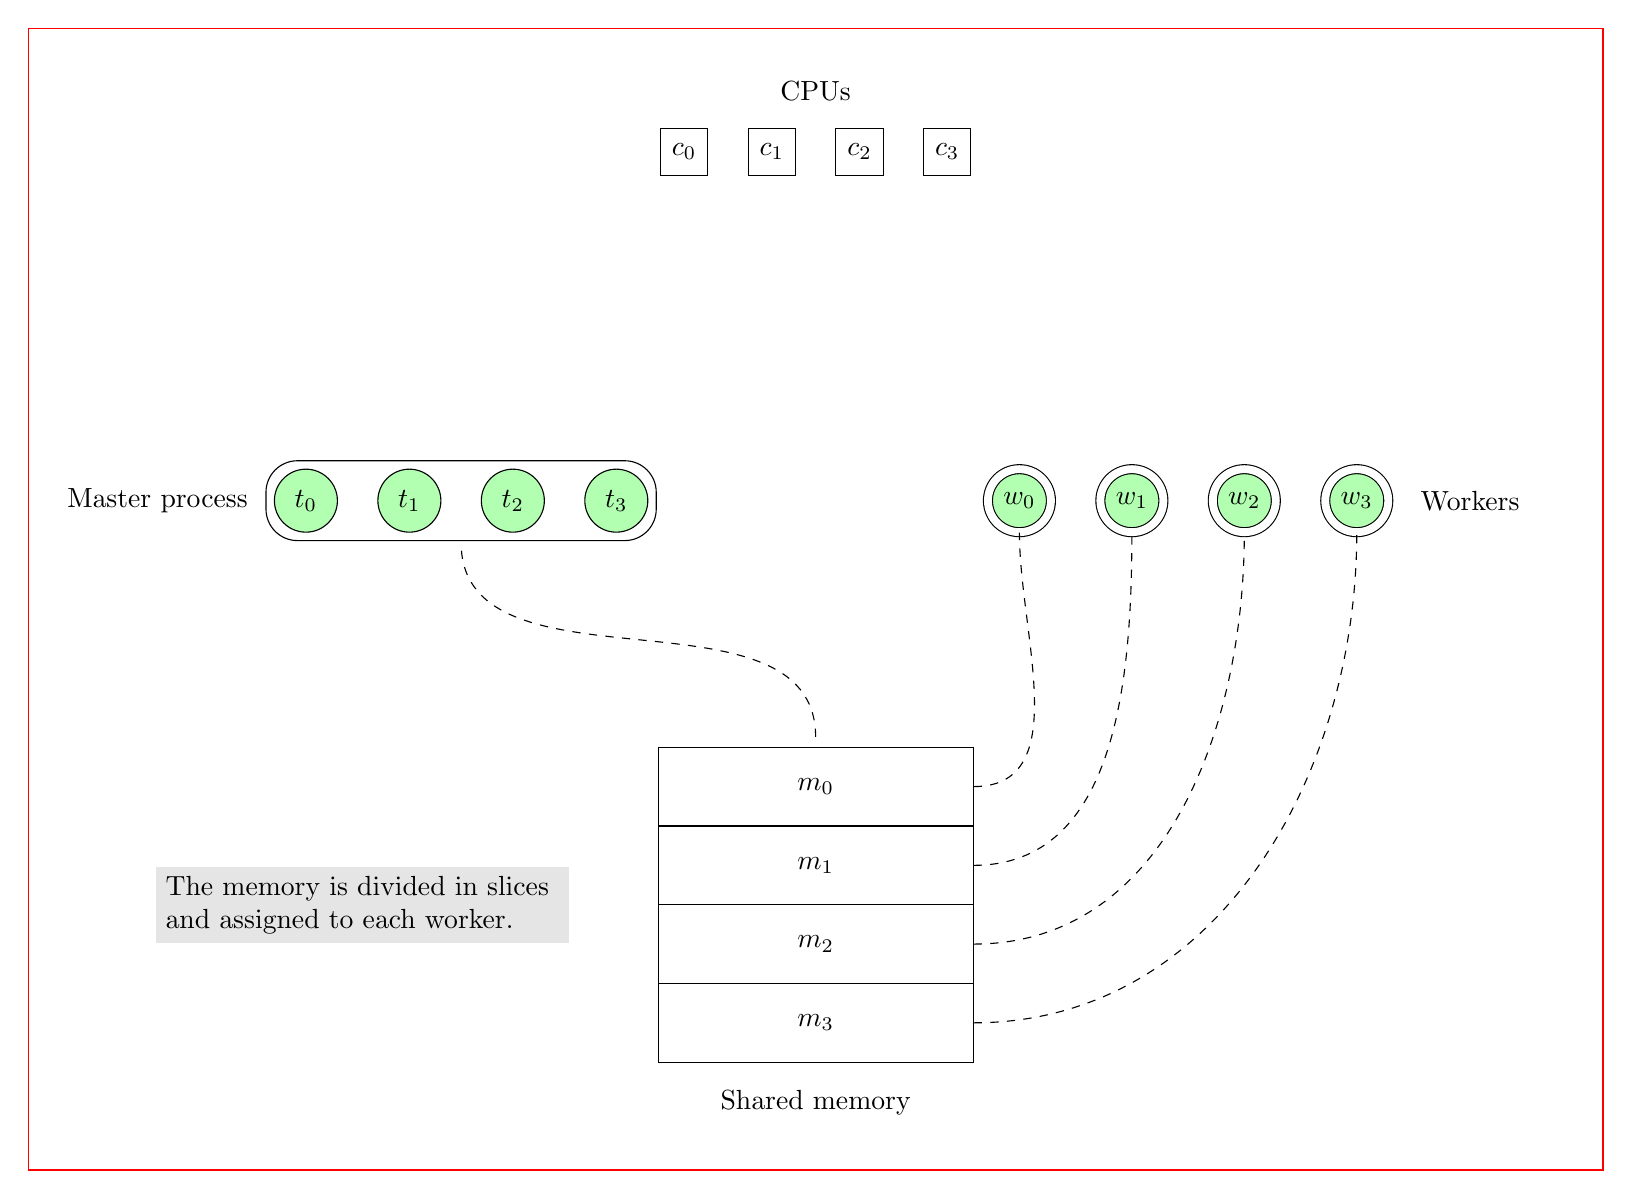
\begin{tikzpicture}[
		>=latex,
	]

	% The center will be the origin
	\coordinate (O) at (0,0);

	% Draw the canvas
	\draw[red] (-10,-8.5) rectangle (10,6);

	% Master process with 4 threads
	\pic[left=2cm of O] {master={running}};

	% Draw the CPUs
	\pic[above=4cm of O] {cpus};

	% Draw the workers
	\pic[right=2cm of O] {workers={running}};

	% Draw shared memory
	\pic[below=3cm of O] {mem};

	\node (text) [fill=gray!20,left=1cm of m,text width=5cm]
		{The memory is divided in slices and assigned to each worker.};

	% Draw shared memory lines
	\foreach \i in {0,...,3}
		\draw[dashed] (m\i) to[out=0,in=-90] (w\i);

	% Draw lines from master to mem
	\draw[dashed] (m.north) to[out=90,in=-90] (t.south);


\end{tikzpicture}
\end{adjustbox}
\end{figure}
\end{frame}

\begin{frame}[fragile]
\begin{figure}[h]
\begin{adjustbox}{max totalsize={\textwidth}{\textheight},center}
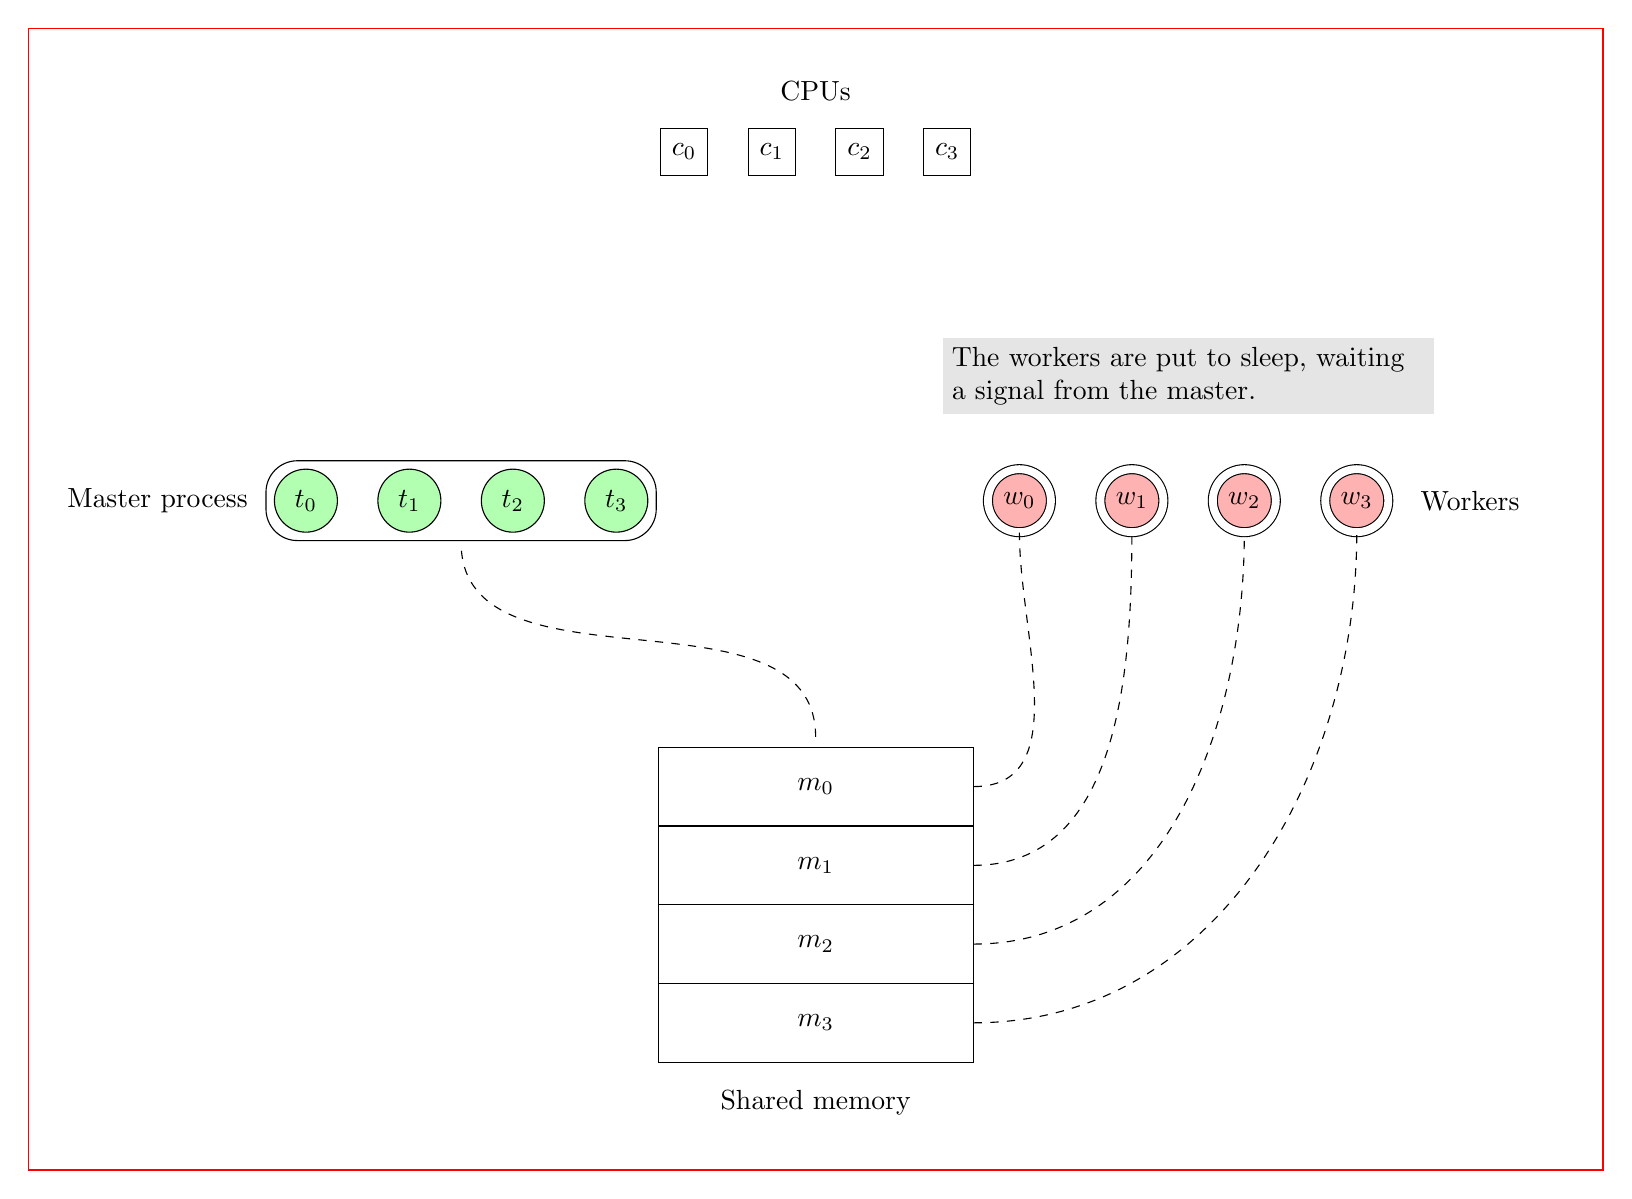
\begin{tikzpicture}[
		>=latex,
	]

	% The center will be the origin
	\coordinate (O) at (0,0);

	% Draw the canvas
	\draw[red] (-10,-8.5) rectangle (10,6);

	% Master process with 4 threads
	\pic[left=2cm of O] {master={running}};

	% Draw the CPUs
	\pic[above=4cm of O] {cpus};

	% Draw the workers
	\pic[right=2cm of O] {workers={stopped}};

	% Draw shared memory
	\pic[below=3cm of O] {mem};

	\node (text) [fill=gray!20,above=0.5cm of w,text width=6cm]
		{The workers are put to sleep, waiting a signal from the master.};

	% Draw shared memory lines
	\foreach \i in {0,...,3}
		\draw[dashed] (m\i) to[out=0,in=-90] (w\i);

	% Draw lines from master to mem
	\draw[dashed] (m.north) to[out=90,in=-90] (t.south);


\end{tikzpicture}
\end{adjustbox}
\end{figure}
\end{frame}

\begin{frame}[fragile]
\begin{figure}[h]
\begin{adjustbox}{max totalsize={\textwidth}{\textheight},center}
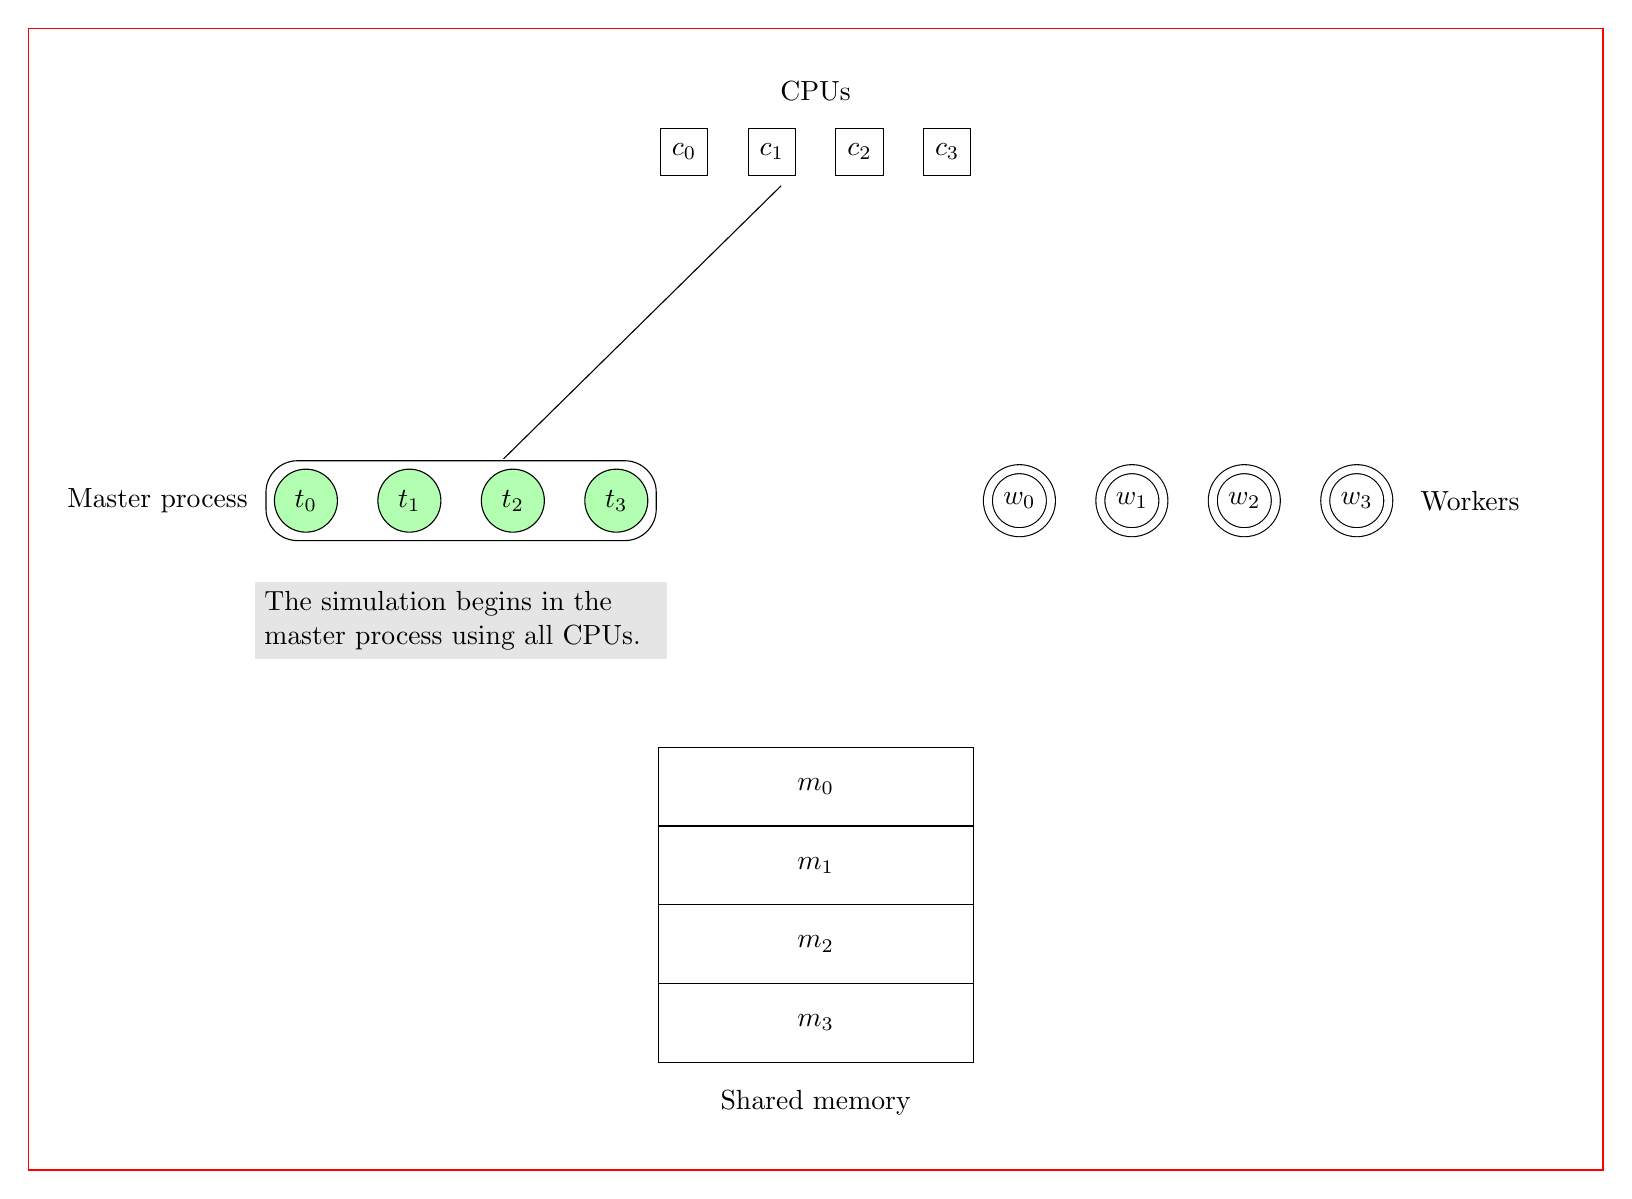
\begin{tikzpicture}[
		>=latex,
	]

	% The center will be the origin
	\coordinate (O) at (0,0);

	% Draw the canvas
	\draw[red] (-10,-8.5) rectangle (10,6);

	% Master process with 4 threads
	\pic[left=2cm of O] {master={fill=green!30}};

	% Draw the CPUs
	\pic[above=4cm of O] {cpus};

	% Draw the workers
	\pic[right=2cm of O] {workers};

	% Draw shared memory
	\pic[below=3cm of O] {mem};

	\node (text) [fill=gray!20,below=0.5cm of t,text width=5cm]
		{The simulation begins in the master process using all CPUs.};

	% Draw arrows from threads to cpus
	%\foreach \i in {0,...,3}
	%	\draw[dashed] (t\i) -- (c\i);

	\draw (t) -- (c);

\end{tikzpicture}
\end{adjustbox}
\end{figure}
\end{frame}

\begin{frame}[fragile]
\begin{figure}[h]
\begin{adjustbox}{max totalsize={\textwidth}{\textheight},center}
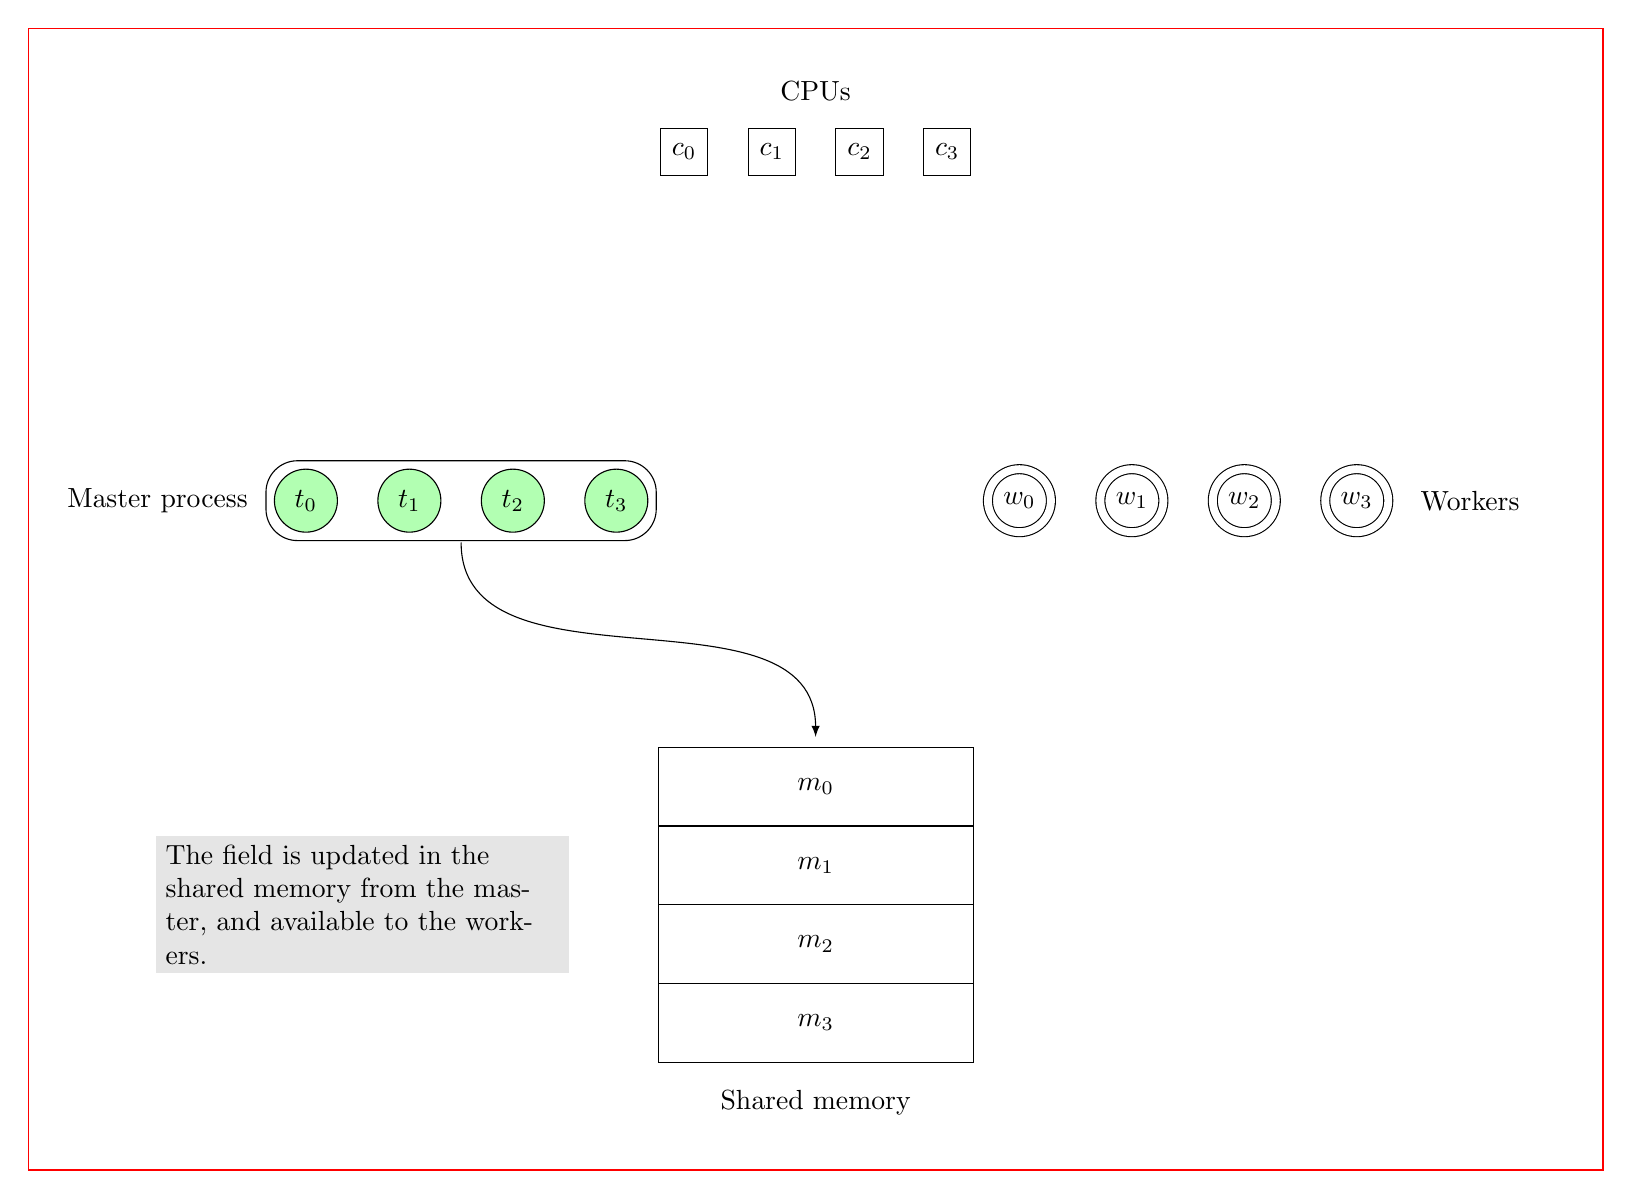
\begin{tikzpicture}[
		>=latex,
	]

	% The center will be the origin
	\coordinate (O) at (0,0);

	% Draw the canvas
	\draw[red] (-10,-8.5) rectangle (10,6);

	% Master process with 4 threads
	\pic[left=2cm of O] {master={fill=green!30}};

	% Draw the CPUs
	\pic[above=4cm of O] {cpus};

	% Draw the workers
	\pic[right=2cm of O] {workers};

	% Draw shared memory
	\pic[below=3cm of O] {mem};

	% Draw lines from master to mem
	\draw[->] (t.south) to[out=-90,in=90] (m.north);
	%\draw[->] (t) -- (m);

	\node (text) [fill=gray!20,left=1cm of m,text width=5cm]
		{The field is updated in the shared memory from the master, and available to 
		the workers.};

\end{tikzpicture}
\end{adjustbox}
\end{figure}
\end{frame}

\begin{frame}[fragile]
\begin{figure}[h]
\begin{adjustbox}{max totalsize={\textwidth}{\textheight},center}
\begin{tikzpicture}[
		>=latex,
	]

	% The center will be the origin
	\coordinate (O) at (0,0);

	% Draw the canvas
	\draw[red] (-10,-8.5) rectangle (10,6);

	% Master process with 4 threads
	\pic[left=2cm of O] {master};

	% Draw the workers
	\pic[right=2cm of O] {workers};

	% Draw the CPUs
	\pic[above=4cm of O] {cpus};

	% Draw arrows from threads to cpus
	\foreach \i in {0,...,3}
		\draw[->,dashed] (t\i) -- (c\i);

	% Draw shared memory
	\pic[below=3cm of O] {mem};

	% Draw shared memory lines
	\foreach \i in {0,...,3}
		\draw[dashed] (m\i) to[out=0,in=-90] (w\i);

	% Brace from memory to the master
	\draw [
		decorate,
		decoration={
			brace,
			mirror,
			amplitude=5mm
		},
		yshift=0pt
	]
	(m0.north west) -- (m3.south west)
		node[black,midway,xshift=-5mm] (mem-brace) {};

	\draw[dashed] (mem-brace) to[out=180,in=-90] (t.south);

	% Label processes
	\node[above=1cm of w0] (process) {Processes};

	\draw[->,shorten >=1.5mm] (process) -- (t3);
	\draw[->,shorten >=0.5mm] (process) -- (w0);
	\draw[->,shorten >=0.5mm] (process) -- (w1);

	% Label threads
	\node[below=2cm of O] (thread) {Threads};
	\draw[->,shorten >=-0.5mm] (thread) -- (w0);
	\draw[->,shorten >=-0.5mm] (thread) -- (t2);
	\draw[->,shorten >=-0.5mm] (thread) -- (t3);

\end{tikzpicture}
\end{adjustbox}
\end{figure}
\end{frame}

\end{document}
